% Hand-written narrative; numbers are macros.
\textbf{Choosing the budget.} The budget matters more than the detector. Going from 10 to 50 alerts
per day raises BudgetAwareConformal's detection rate from \DROursBA{} to \DROursBB{} and Isolation
Forest's from \DRIFBA{} to \DRIFBB{}, while precision falls only from \POursBA{} to \POursBB{}
(Fig.~\ref{fig:precision}). Because precision is already far below its ceiling, the extra alerts are
cheap in relative terms; a team that can review 50 alerts a day gains far more from the detector
than one limited to 10.

\textbf{Precision or coverage.} At 10 alerts per day LOF and the autoencoder cover a similar share of
insiders but raise roughly twice as many false alerts per true one. Where analyst time is the
binding constraint, the per-user detector is the better choice; where missing an insider is far
costlier than reviewing false alerts, a density baseline is a reasonable complement, and the two
could share one queue.

\textbf{Working the queue by explanation.} Ranking only by score ignores information the detector
already produces. Since volume-explained alerts are true several times more often than the rest
(Table~\ref{tab:family}), an analyst can triage those first; identity-only deviations (new PCs) were
never malicious in our test windows.

\textbf{Organisation size and cost.} The budget is fixed per day, so the same 10 alerts cover a
larger share of a smaller organisation. On random samples of \NUsersSmall{} and \NUsersMid{} users the
detection rate at 10 alerts per day is \DRSweepOursSmall{} and \DRSweepOursMid{} for our detector
(Isolation Forest \DRSweepIFSmall{} and \DRSweepIFMid), against \DRSweepOursFull{} on all
\NUsersFull{} users (Fig.~\ref{fig:scale}; means over runs, hence slightly different from the
insider-pooled estimate of Table~\ref{tab:main}). Fitting and scoring one test window on all users takes
\SecsOurs\,s for BudgetAwareConformal, against \SecsIF\,s for Isolation Forest, \SecsLOF\,s for LOF
and \SecsAE\,s for the autoencoder.

\begin{figure}[t]
\centering
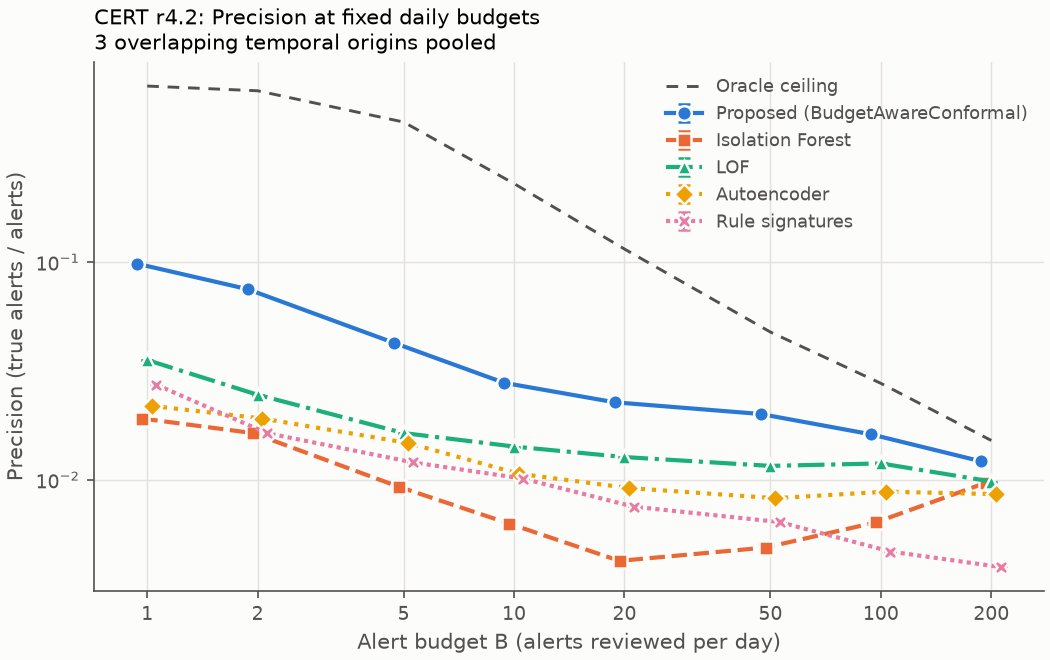
\includegraphics[width=\columnwidth]{figures/precision_vs_budget.png}
\caption{Precision against the daily alert budget (log scales) with the oracle ceiling, CERT r4.2
test windows.}
\label{fig:precision}
\end{figure}

\begin{figure}[t]
\centering
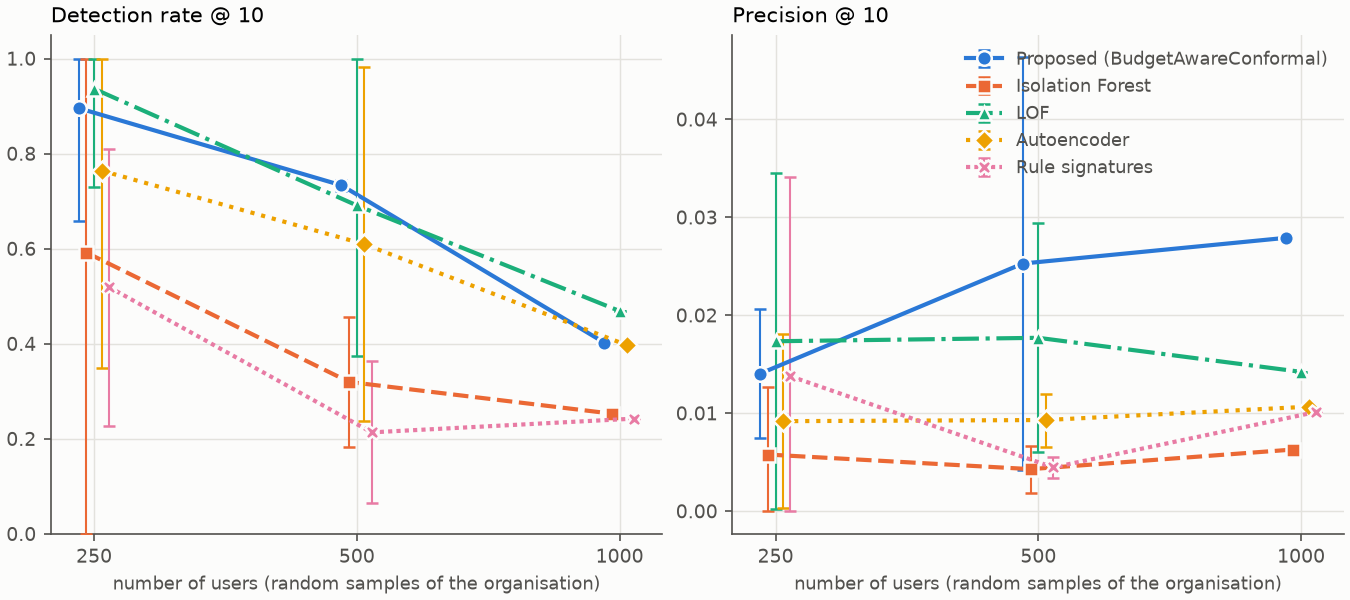
\includegraphics[width=\columnwidth]{figures/sweep_principals.png}
\caption{Detection rate and precision at 10 alerts/day on random samples of the organisation (three
samples per size; 95\% $t$-interval over samples).}
\label{fig:scale}
\end{figure}
